\section{Integración con los servicios}\label{sec:integracion-servicios}

Una vez configurado el balanceador, se realizó la conexión de los servicios con FreeIPA. Para ello, se utilizó la identidad asociada al balanceador de carga, representada mediante el nombre virtual ipa.grid.uniquindio.edu.co. Esta identidad permite que los servicios integrados utilicen un único punto de acceso al directorio, delegando en HAProxy la distribución de las solicitudes entre el servidor principal y la réplica, de acuerdo con su disponibilidad. De esta manera, los servicios no necesitan establecer una dependencia directa con un servidor específico de FreeIPA, sino que utilizan la identidad común definida para la solución.

\subsection{OpenVPN}\label{subsec:integracion-openvpn}

Para realizar la integración de OpenVPN con el servicio de gestión de identidades FreeIPA mediante el protocolo \ac{LDAP}, fue necesario instalar previamente el complemento openvpn-auth-ldap. Este componente permite que el servidor OpenVPN utilice un directorio \ac{LDAP} como fuente para la autenticación de los usuarios, delegando en FreeIPA la validación de las credenciales y la aplicación de las reglas de autorización definidas. Por esta razón, como primer paso se realizó la instalación del complemento mediante el gestor de paquetes del sistema operativo, como se observa en la \autoref{fig:instalacion-openvpn-autenticacion-ldap}.

\begin{figure}[H]
	\centering
	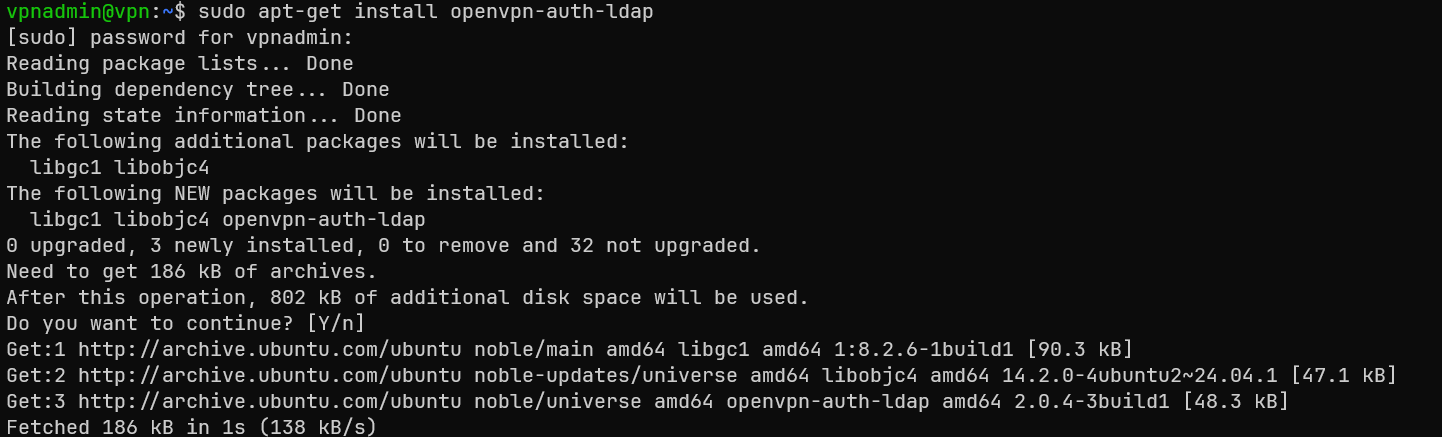
\includegraphics[width=0.8\textwidth]{mainmatter/II-desarrollo-metodologico/implementacion/imagenes/instalacion-openvpn-autenticacion-ldap.png}
	\caption{Instalación del complemento openvpn-auth-ldap}
	\label{fig:instalacion-openvpn-autenticacion-ldap}
\end{figure}

Para establecer la conexión \ac{LDAPS} entre OpenVPN y FreeIPA, primero fue necesario obtener el certificado de la autoridad certificadora (\acs{CA}) utilizada por FreeIPA. Desde la interfaz de línea de comandos del servidor FreeIPA, este certificado se encuentra disponible en la ruta /etc/ipa/ca.crt, desde donde puede ser copiado al servidor que ejecuta OpenVPN.

Como alternativa, el certificado puede obtenerse mediante la interfaz web de FreeIPA utilizando la URL \nolinkurl{https://ipa.grid.uniquindio.edu.co/ipa/config/ca.crt}. Al acceder a esta dirección se obtiene directamente el certificado de la autoridad certificadora utilizado por FreeIPA.

Una vez obtenido el certificado, se creó el archivo ca.crt en la ruta \path{/etc/openvpn/auth/ca.crt} del servidor OpenVPN, almacenando en este el certificado de la autoridad certificadora de FreeIPA. La disposición del certificado en esta ubicación permite utilizarlo como referencia para la validación de la conexión segura con el servicio \ac{LDAP} y constituye un elemento necesario para los siguientes pasos de configuración del complemento openvpn-auth-ldap. El archivo ca.crt en la ubicación correspondiente se muestra en la \autoref{fig:ubicacion-certificado-ca-openvpn}.

\begin{figure}[H]
	\centering
	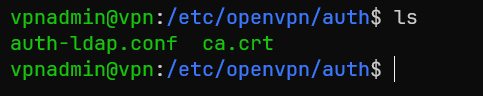
\includegraphics[width=0.8\textwidth]{mainmatter/II-desarrollo-metodologico/implementacion/imagenes/ubicacion-certificado-ca-openvpn.png}
	\caption{Archivo ca.crt ubicado en /etc/openvpn/auth/}
	\label{fig:ubicacion-certificado-ca-openvpn}
\end{figure}

Una vez instalado el complemento y ubicado el certificado de la autoridad certificadora en la ruta correspondiente, se procedió a configurar los parámetros necesarios para establecer la comunicación entre OpenVPN y FreeIPA. Esta configuración se realiza mediante el archivo auth-ldap.conf, utilizado por openvpn-auth-ldap para definir tanto los parámetros de conexión al directorio como los criterios mediante los cuales se buscan y autorizan los usuarios.

El paquete proporciona un archivo de configuración de ejemplo ubicado en \path{/usr/share/doc/openvpn-auth-ldap/examples/auth-ldap.conf}, el cual contiene diferentes parámetros para establecer una conexión \ac{LDAP}. A partir de este archivo se seleccionaron y adaptaron únicamente los parámetros necesarios para la infraestructura implementada. La configuración resultante se presenta en la \autoref{fig:configuracion-openvpn-autenticacion-ldap}.

\begin{figure}[H]
	\centering
	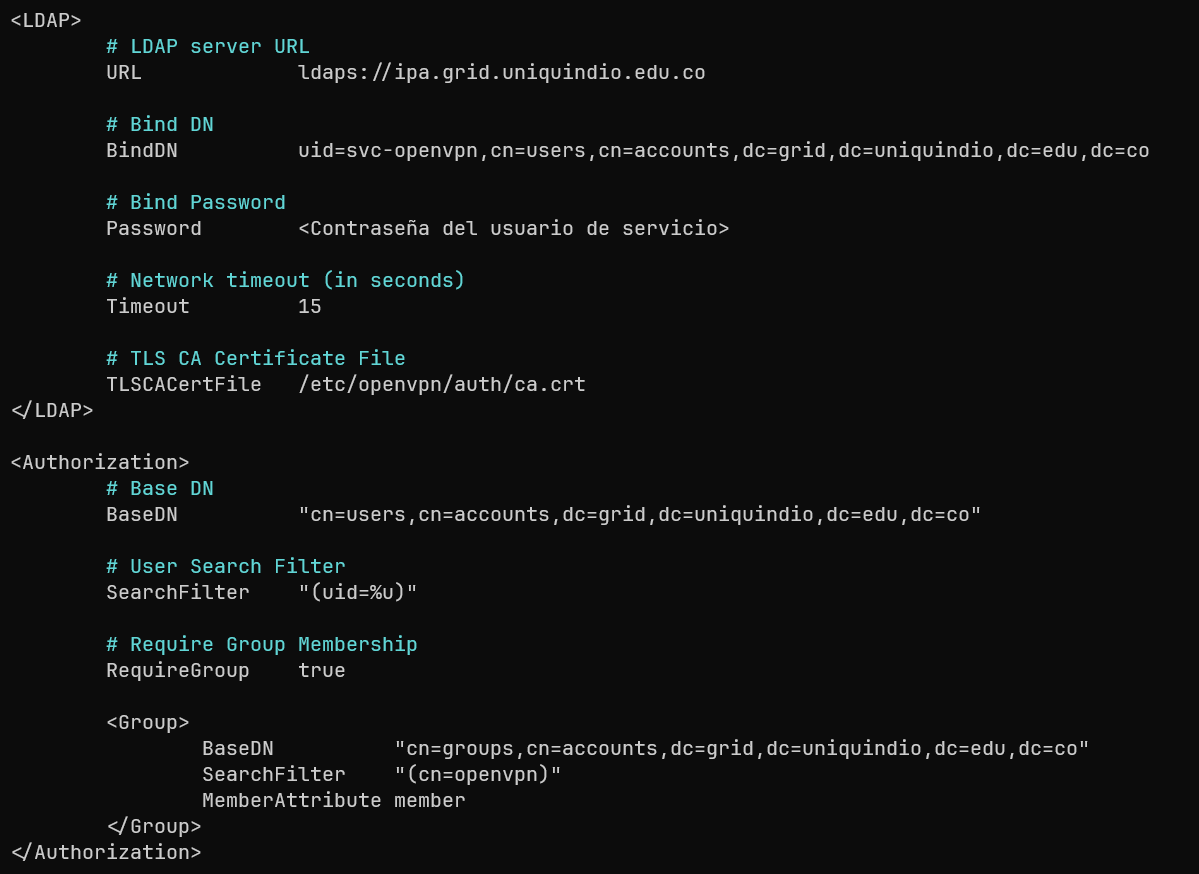
\includegraphics[width=0.8\textwidth]{mainmatter/II-desarrollo-metodologico/implementacion/imagenes/configuracion-openvpn-autenticacion-ldap.png}
	\caption{Configuración del complemento openvpn-auth-ldap para la integración con FreeIPA}
	\label{fig:configuracion-openvpn-autenticacion-ldap}
\end{figure}

Dentro del bloque \texttt{<LDAP>} se definieron inicialmente los parámetros relacionados con la conexión al servicio de directorio. El parámetro \texttt{URL} se configuró con el valor \nolinkurl{ldaps://ipa.grid.uniquindio.edu.co}, utilizando el nombre virtual asignado al servicio. De esta manera, OpenVPN no establece una dependencia directa con los nodos \texttt{ipa1} o \texttt{ipa2}, sino que dirige las solicitudes hacia HAProxy, el cual posteriormente determina cuál de los servidores FreeIPA disponibles atenderá la conexión.

Para realizar las consultas al directorio se configuró el parámetro \texttt{BindDN} con la cuenta de servicio \texttt{svc-openvpn}, utilizando su \ac{DN} completo:

\begin{center}
	\texttt{uid=svc-openvpn,cn=users,cn=accounts,dc=grid,dc=uniquindio,dc=co}
\end{center}

Esta cuenta se utiliza exclusivamente para que el servicio pueda realizar las consultas necesarias en FreeIPA y se encuentra separada de las cuentas personales de los usuarios. Su contraseña se establece mediante el parámetro \texttt{Password}. De esta manera, el complemento dispone de una identidad propia para realizar las operaciones de consulta contra el directorio.

También se estableció un tiempo máximo de espera de 15 segundos mediante el parámetro \texttt{Timeout}. Este valor determina cuánto tiempo esperará el complemento por una respuesta del servidor \ac{LDAP} antes de considerar que la comunicación no se ha completado correctamente.

A diferencia del archivo de ejemplo, en la configuración implementada no fue necesario habilitar explícitamente \texttt{TLSEnable}, debido a que la conexión se realiza directamente mediante \ac{LDAPS}, utilizando el esquema \texttt{ldaps://}. Para validar la identidad del servidor durante el establecimiento de la conexión segura, se especificó mediante \texttt{TLSCACertFile} el certificado de la autoridad certificadora de FreeIPA ubicado en \texttt{/etc/openvpn/auth/ca.crt}. Esto permite que OpenVPN pueda verificar que el certificado presentado por el servicio \ac{LDAP} es emitido por una autoridad de confianza.

En el bloque \texttt{<Authorization>} se definieron los parámetros encargados de determinar cómo se localizan y autorizan los usuarios dentro del directorio. El parámetro \texttt{BaseDN} se estableció en \texttt{cn=users,cn=accounts,dc=grid,dc=uniquindio,dc=co}, limitando las búsquedas de usuarios a la rama correspondiente a las cuentas de usuario de FreeIPA.

El parámetro \texttt{SearchFilter} se configuró como \texttt{(uid=\%u)}. El valor \texttt{\%u} es sustituido por el nombre de usuario proporcionado durante el inicio de sesión en OpenVPN. De esta manera, el complemento construye una búsqueda \ac{LDAP} que permite localizar dentro de FreeIPA la cuenta correspondiente al usuario que intenta autenticarse.

Además de validar que el usuario exista en el directorio, se estableció \texttt{RequireGroup true}, haciendo que la pertenencia a un grupo sea un requisito para completar la autorización. Esta configuración permite utilizar los grupos de FreeIPA como mecanismo de control de acceso al servicio OpenVPN, evitando que cualquier usuario registrado en el directorio pueda acceder automáticamente al servicio.

Para aplicar esta restricción se configuró el bloque \texttt{<Group>}. En este se estableció como \texttt{BaseDN} la rama \texttt{cn=groups,cn=accounts,dc=grid,dc=uniquindio,dc=co}, correspondiente a los grupos administrados por FreeIPA. El parámetro \texttt{SearchFilter} se configuró como \texttt{(cn=openvpn)}, por lo que el complemento busca específicamente el grupo \texttt{openvpn}.

Finalmente, se estableció \texttt{MemberAttribute member}, indicando el atributo utilizado por FreeIPA para determinar la pertenencia de los usuarios al grupo. En consecuencia, para que un usuario pueda autenticarse mediante OpenVPN no es suficiente con que sus credenciales sean válidas: también debe pertenecer al grupo \texttt{openvpn} definido previamente en FreeIPA.

De esta manera, la configuración implementada establece un flujo en el que Open\-VPN recibe las credenciales del usuario, \texttt{openvpn-auth-ldap} realiza las consultas contra FreeIPA mediante el nombre virtual \texttt{ipa.grid.uniquindio.edu.co}, HAProxy distribuye la conexión entre los servidores disponibles y FreeIPA valida tanto la existencia del usuario como su pertenencia al grupo autorizado para utilizar el servicio. Esto permite integrar la autenticación y autorización de OpenVPN con la gestión centralizada de identidades implementada en la infraestructura.

Una vez finalizada la configuración del archivo \texttt{auth-ldap.conf}, se procedió a habilitar el complemento en el servidor OpenVPN. Para ello, fue necesario modificar el archivo de configuración del servidor, ubicado en \path{/etc/openvpn/server/server.conf}, agregando la directiva \texttt{plugin}. Esta permite indicar a OpenVPN qué complemento debe cargar y especificar el archivo de configuración que contiene los parámetros necesarios para la conexión con FreeIPA. La línea agregada fue la siguiente:

\begin{center}
	\texttt{plugin /usr/lib/openvpn/openvpn-auth-ldap.so /etc/openvpn/auth/auth-ldap.conf}
\end{center}

En la \autoref{fig:activacion-openvpn-autenticacion-ldap} se observa la incorporación de esta directiva en el archivo de configuración del servidor OpenVPN.

\begin{figure}[H]
	\centering
	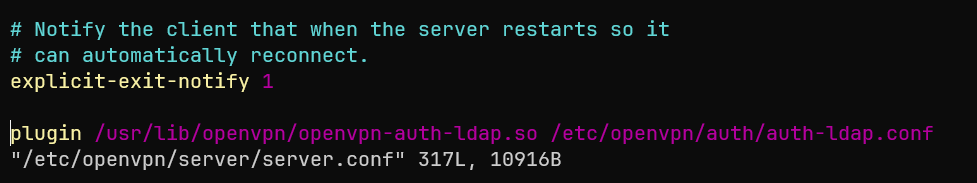
\includegraphics[width=0.8\textwidth]{mainmatter/II-desarrollo-metodologico/implementacion/imagenes/activacion-openvpn-autenticacion-ldap.png}
	\caption{Activación del complemento openvpn-auth-ldap en la configuración del servidor OpenVPN}
	\label{fig:activacion-openvpn-autenticacion-ldap}
\end{figure}

Finalmente, para que los clientes de OpenVPN puedan proporcionar las credenciales utilizadas para su autenticación mediante FreeIPA, fue necesario modificar el archivo de configuración .ovpn utilizado por el cliente. Para ello, se agregó la directiva auth-user-pass, la cual indica al cliente que debe solicitar las credenciales de usuario y contraseña durante el proceso de conexión. Esta configuración es necesaria para que las credenciales sean enviadas al servidor OpenVPN y puedan ser procesadas por el complemento openvpn-auth-ldap. En caso de no incluir esta directiva, el cliente no solicitará las credenciales requeridas y la autenticación mediante \ac{LDAP} no podrá completarse. La incorporación de la directiva auth-user-pass en el archivo de configuración del cliente se observa en la \autoref{fig:configuracion-autenticacion-cliente-openvpn}.

\begin{figure}[H]
	\centering
	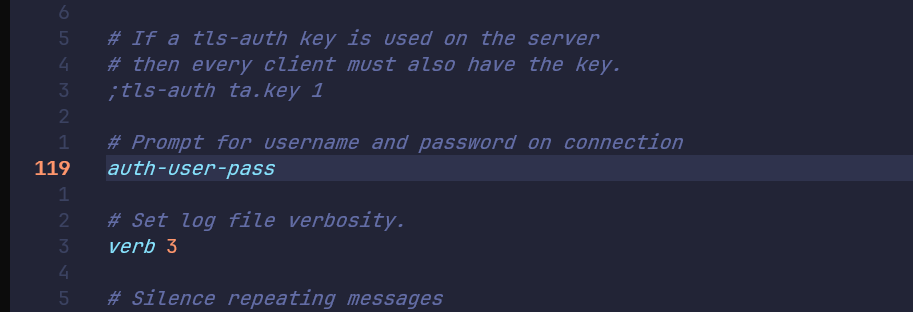
\includegraphics[width=0.8\textwidth]{mainmatter/II-desarrollo-metodologico/implementacion/imagenes/configuracion-autenticacion-cliente-openvpn.png}
	\caption{Configuración de autenticación mediante usuario y contraseña en el cliente OpenVPN}
	\label{fig:configuracion-autenticacion-cliente-openvpn}
\end{figure}

\subsection{OpenProject}\label{subsec:integracion-openproject}

Para realizar la integración de OpenProject con el servicio de directorio, fue necesario configurar una conexión \ac{LDAP} desde la interfaz de administración de la plataforma. Para acceder a esta configuración, se ingresó al menú Perfil → Administración → Autenticación → Conexiones \ac{LDAP}, desde donde es posible administrar las conexiones con servidores de directorio.

En esta sección se creó una nueva conexión \ac{LDAP}, en cuyo formulario se definieron inicialmente los parámetros básicos de comunicación con el servicio, incluyendo el nombre asignado a la conexión, el host o dirección del servicio \ac{LDAP} y el puerto utilizado para establecer la comunicación. En este caso, la conexión se configuró utilizando la identidad del servicio definida mediante \nolinkurl{ipa.grid.uniquindio.edu.co}, permitiendo que OpenProject utilice el punto de acceso proporcionado por HAProxy en lugar de establecer una conexión directa con un servidor específico de FreeIPA. Los parámetros iniciales de la conexión \ac{LDAP} configurada se presentan en la \autoref{fig:configuracion-inicial-ldap-openproject}.

\begin{figure}[H]
	\centering
	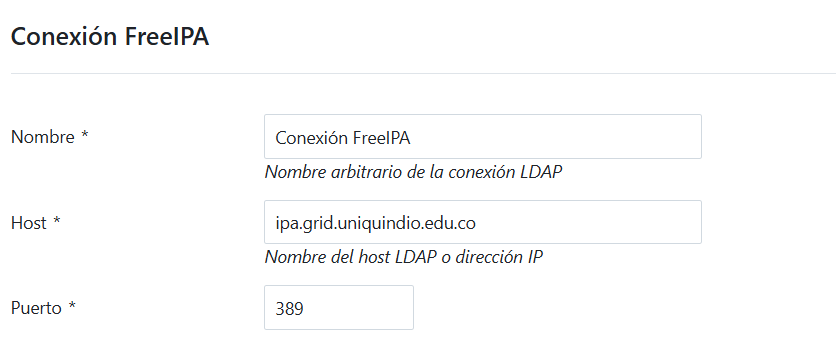
\includegraphics[width=0.8\textwidth]{mainmatter/II-desarrollo-metodologico/implementacion/imagenes/configuracion-inicial-ldap-openproject.png}
	\caption{Configuración inicial de la conexión \acs{LDAP} en OpenProject}
	\label{fig:configuracion-inicial-ldap-openproject}
\end{figure}

Posteriormente, se configuraron los parámetros relacionados con la seguridad de la conexión \ac{LDAP}. OpenProject permite seleccionar entre tres modalidades de conexión: sin cifrado, STARTTLS y \ac{LDAPS}. Debido a que el servicio de directorio se encuentra configurado para admitir tanto conexiones STARTTLS como \ac{LDAPS}, se seleccionó STARTTLS, opción recomendada por OpenProject para establecer una conexión \ac{LDAP} protegida mediante \ac{TLS}.

Adicionalmente, se habilitó la opción de validación del certificado \ac{SSL}, con el propósito de verificar la identidad del servidor durante el establecimiento de la conexión y mantener la seguridad de las comunicaciones. Al activar esta opción, OpenProject permite proporcionar el certificado de la autoridad certificadora utilizada para validar el certificado presentado por el servicio \ac{LDAP}. Para este caso, se incorporó el certificado de la \acs{CA} de FreeIPA previamente obtenido, permitiendo que OpenProject pueda validar la cadena de confianza al establecer la conexión mediante ipa.grid.uniquindio.edu.co. La configuración de seguridad \ac{TLS} y validación del certificado se muestra en la \autoref{fig:seguridad-tls-certificado-openproject}.

\begin{figure}[H]
	\centering
	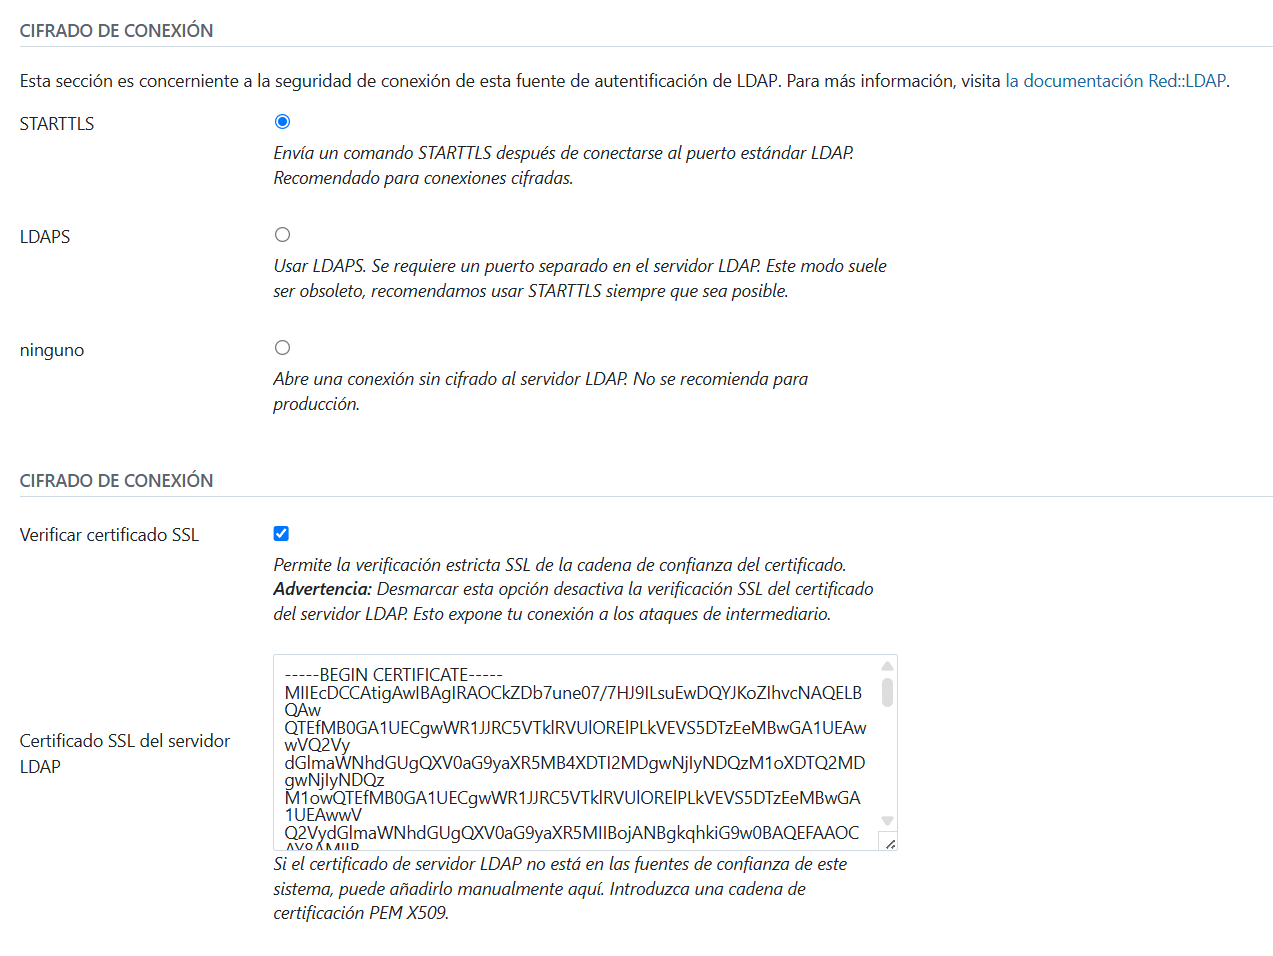
\includegraphics[width=0.8\textwidth]{mainmatter/II-desarrollo-metodologico/implementacion/imagenes/seguridad-tls-certificado-openproject.png}
	\caption{Configuración de seguridad \acs{TLS} y validación del certificado de la conexión \acs{LDAP}}
	\label{fig:seguridad-tls-certificado-openproject}
\end{figure}

El siguiente apartado corresponde a la configuración de la cuenta de servicio previamente creada para la integración con FreeIPA. Esta cuenta permite que OpenProject realice las consultas necesarias en el directorio \ac{LDAP} y, para ello, se deben proporcionar las credenciales con las que se establecerá dicha comunicación. En este formulario se definieron el \ac{DN} de la cuenta de servicio y su respectiva contraseña. El \ac{DN} utilizado fue \nolinkurl{uid=svc-openproject,cn=users,cn=accounts,dc=grid,dc=uniquindio,dc=co}, correspondiente a la cuenta de servicio creada específicamente para OpenProject. La configuración de la cuenta de servicio para la conexión \ac{LDAP} se presenta en la \autoref{fig:cuenta-servicio-ldap-openproject}.

\begin{figure}[H]
	\centering
	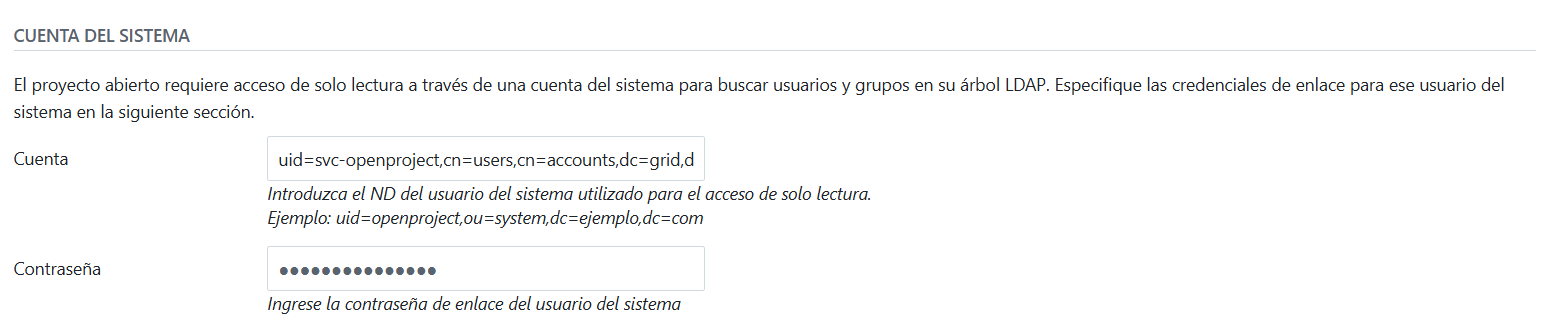
\includegraphics[width=0.8\textwidth]{mainmatter/II-desarrollo-metodologico/implementacion/imagenes/cuenta-servicio-ldap-openproject.png}
	\caption{Configuración de la cuenta de servicio para la conexión \acs{LDAP} de OpenProject}
	\label{fig:cuenta-servicio-ldap-openproject}
\end{figure}

Posteriormente, se configuraron los parámetros correspondientes a los detalles de búsqueda dentro del directorio \ac{LDAP}. En el campo \texttt{Base DN} se estableció \nolinkurl{dc=grid,dc=uniquindio,dc=edu,dc=co}, correspondiente a la raíz del directorio de FreeIPA. Esta configuración permite que OpenProject realice las búsquedas de usuarios y grupos dentro del dominio \ac{LDAP} definido para la infraestructura.

Para limitar los usuarios que pueden ser sincronizados y autenticarse mediante esta conexión, se definió el filtro \nolinkurl{(memberOf=cn=openproject,cn=groups,cn=accounts,dc=grid,dc=uniquindio,dc=edu,dc=co)} el cual está asociado al grupo openproject. De esta manera, OpenProject no considera de forma indiscriminada todas las cuentas existentes en FreeIPA, sino únicamente aquellas que cumplen con la pertenencia al grupo destinado al servicio. Esta configuración permite utilizar los grupos definidos previamente en FreeIPA como mecanismo de control de acceso para OpenProject.

Asimismo, se mantuvo habilitada la opción de creación automática de usuarios, permitiendo que una cuenta de FreeIPA que cumpla con los criterios establecidos pueda ser creada automáticamente en OpenProject durante su primera autenticación. Esto evita tener que crear manualmente en OpenProject cada una de las cuentas que ya se encuentran administradas desde el servicio centralizado de identidades. Los parámetros de búsqueda de usuarios configurados se observan en la \autoref{fig:base-dn-busqueda-openproject}.

\begin{figure}[H]
	\centering
	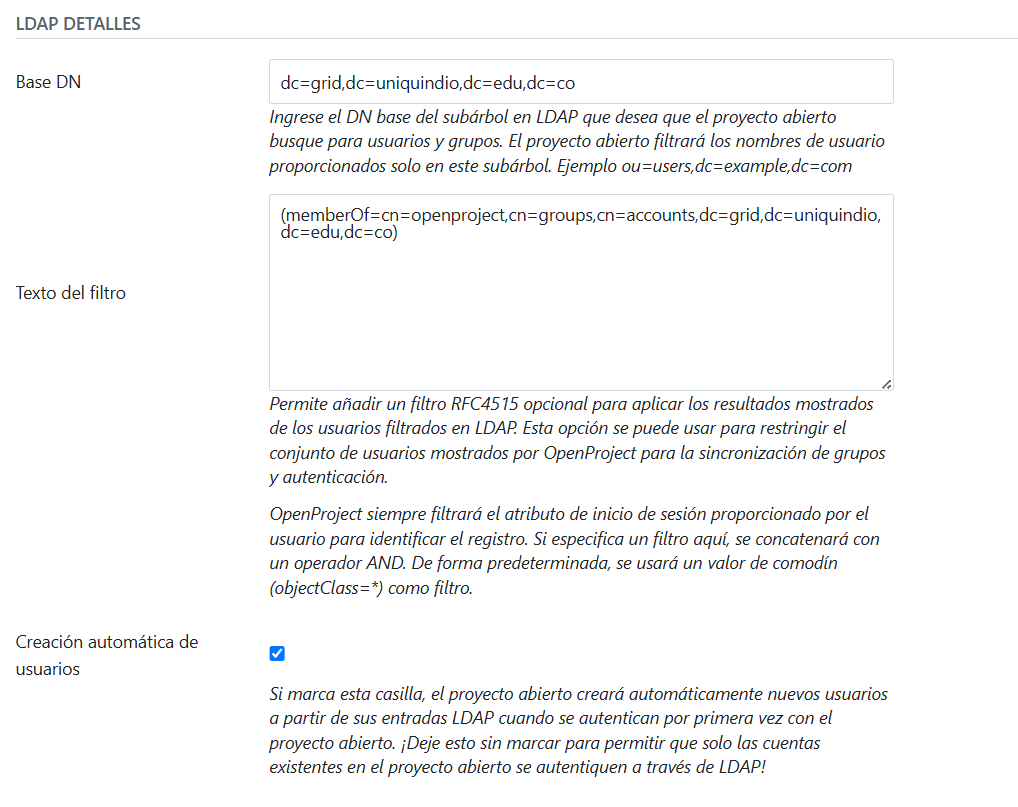
\includegraphics[width=0.8\textwidth]{mainmatter/II-desarrollo-metodologico/implementacion/imagenes/base-dn-busqueda-openproject.png}
	\caption{Configuración de la base \acs{DN} y los criterios de búsqueda de usuarios en OpenProject}
	\label{fig:base-dn-busqueda-openproject}
\end{figure}

Finalmente, se realizó el mapeo de atributos, mediante el cual se estableció la correspondencia entre los atributos definidos en las cuentas de usuario de FreeIPA y los campos utilizados por OpenProject. Esta configuración permite que, al crear o sincronizar un usuario a partir de una entrada \ac{LDAP}, OpenProject pueda identificar y asignar correctamente la información de la cuenta.

Para el nombre de usuario se definió el atributo uid, utilizado como identificador de inicio de sesión. Para el campo Nombre se estableció givenName, mientras que para Apellido se configuró sn. Finalmente, para el Correo electrónico se utilizó el atributo mail. Estos atributos corresponden a la información almacenada en las cuentas de usuario de FreeIPA y permiten que OpenProject complete los datos básicos del usuario a partir del directorio centralizado.

El campo Administrador se dejó sin configurar, debido a que no se utilizó un atributo \ac{LDAP} para determinar directamente los privilegios administrativos dentro de OpenProject. El mapeo de atributos configurado para la integración se presenta en la \autoref{fig:mapeo-atributos-ldap-openproject}.

\begin{figure}[H]
	\centering
	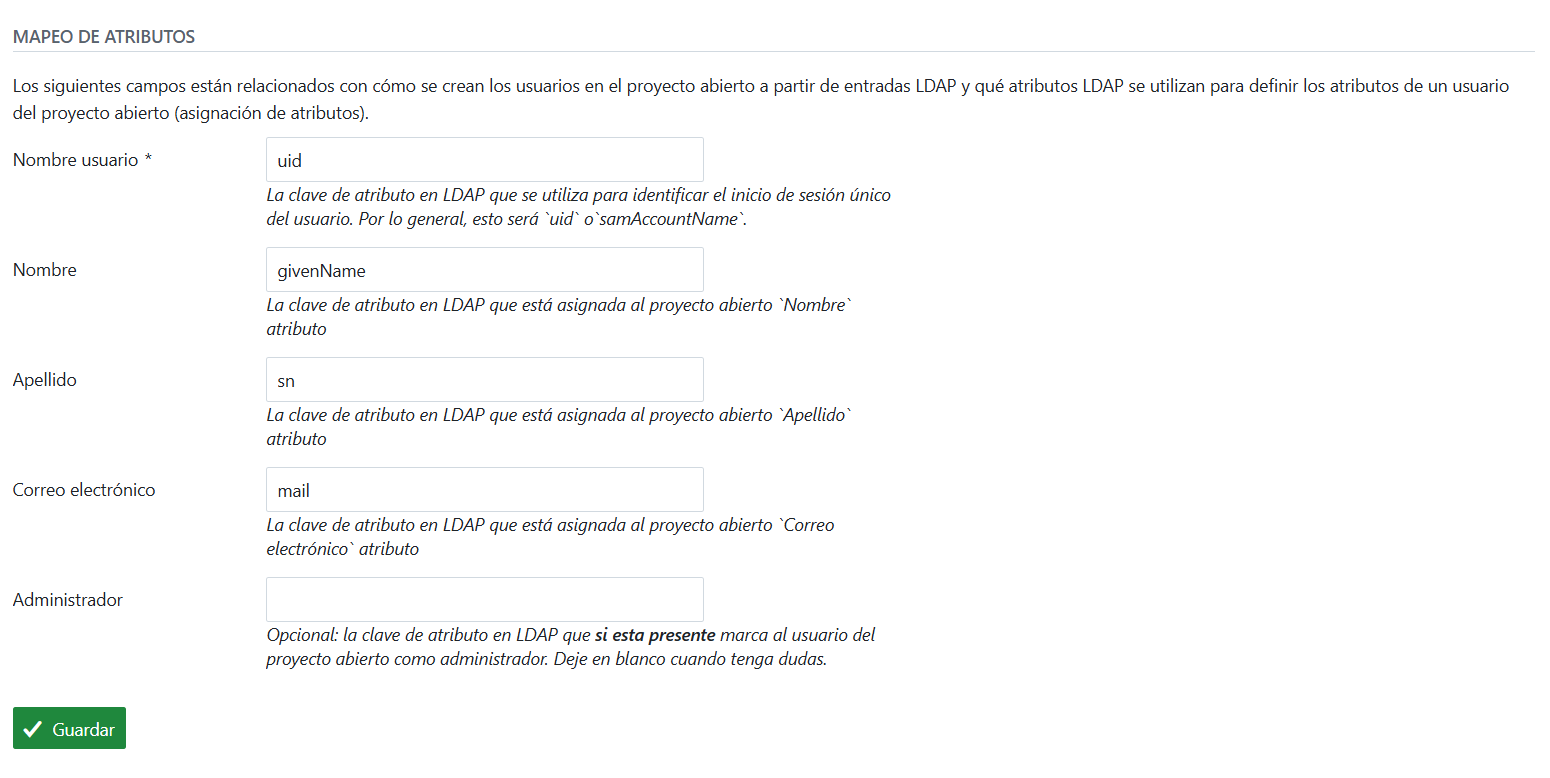
\includegraphics[width=0.8\textwidth]{mainmatter/II-desarrollo-metodologico/implementacion/imagenes/mapeo-atributos-ldap-openproject.png}
	\caption{Mapeo de atributos \acs{LDAP} para los usuarios de OpenProject}
	\label{fig:mapeo-atributos-ldap-openproject}
\end{figure}

Una vez guardada la configuración de la conexión \ac{LDAP}, OpenProject permite realizar una prueba para verificar la comunicación con el servicio de directorio y validar los parámetros configurados. Al ejecutar esta prueba, la plataforma confirmó que la conexión con el servicio FreeIPA se estableció correctamente, mostrando el mensaje «Conexión exitosa». Este resultado permite comprobar que los parámetros de conexión, seguridad y autenticación definidos previamente son aceptados por el servidor de directorio. La conexión \ac{LDAP} configurada y el resultado satisfactorio de la prueba de conectividad se muestran en la \autoref{fig:validacion-conexion-openproject-freeipa}.

\begin{figure}[H]
	\centering
	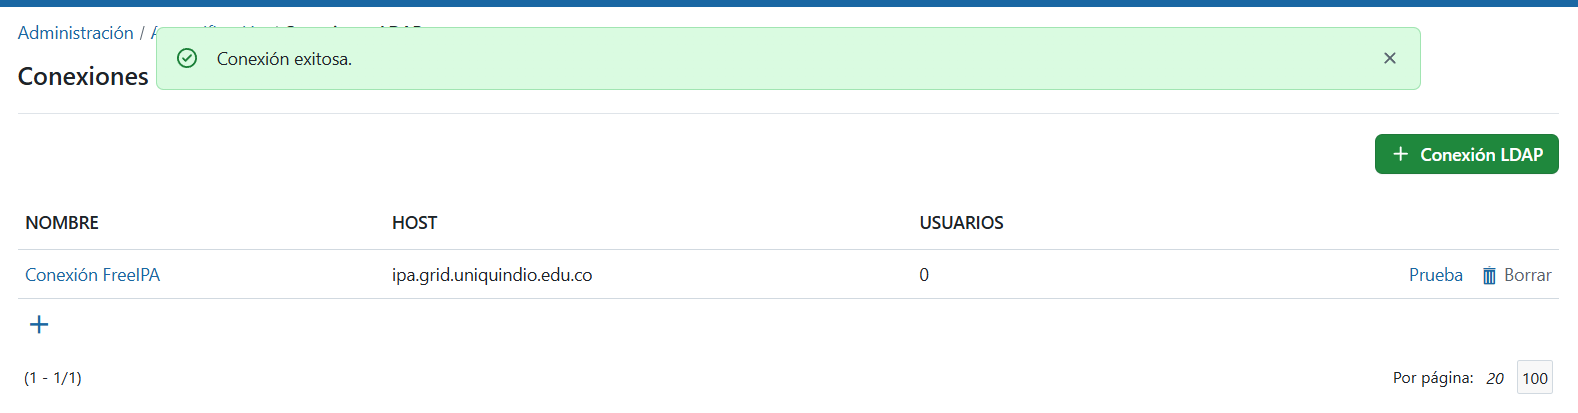
\includegraphics[width=0.8\textwidth]{mainmatter/II-desarrollo-metodologico/implementacion/imagenes/validacion-conexion-openproject-freeipa.png}
	\caption{Validación de la conexión entre OpenProject y FreeIPA}
	\label{fig:validacion-conexion-openproject-freeipa}
\end{figure}

\subsection{Xen Orchestra}\label{subsec:integracion-xen-orchestra}

Como primer paso, se procede a habilitar el complemento \ac{LDAP} en Xen Orchestra. Para ello, se ingresa a Configuración → Complementos (Plugins) y se localiza el complemento correspondiente a la autenticación \ac{LDAP}. Para habilitarlo, es necesario crear previamente una configuración asociada al complemento y guardarla. Una vez habilitado, se pueden establecer los diferentes parámetros requeridos para su integración con el servicio de directorio, los cuales son configurados en los siguientes pasos. El complemento \ac{LDAP} disponible en la sección de complementos se observa en la \autoref{fig:complemento-ldap-xen-orchestra}.

\begin{figure}[H]
	\centering
	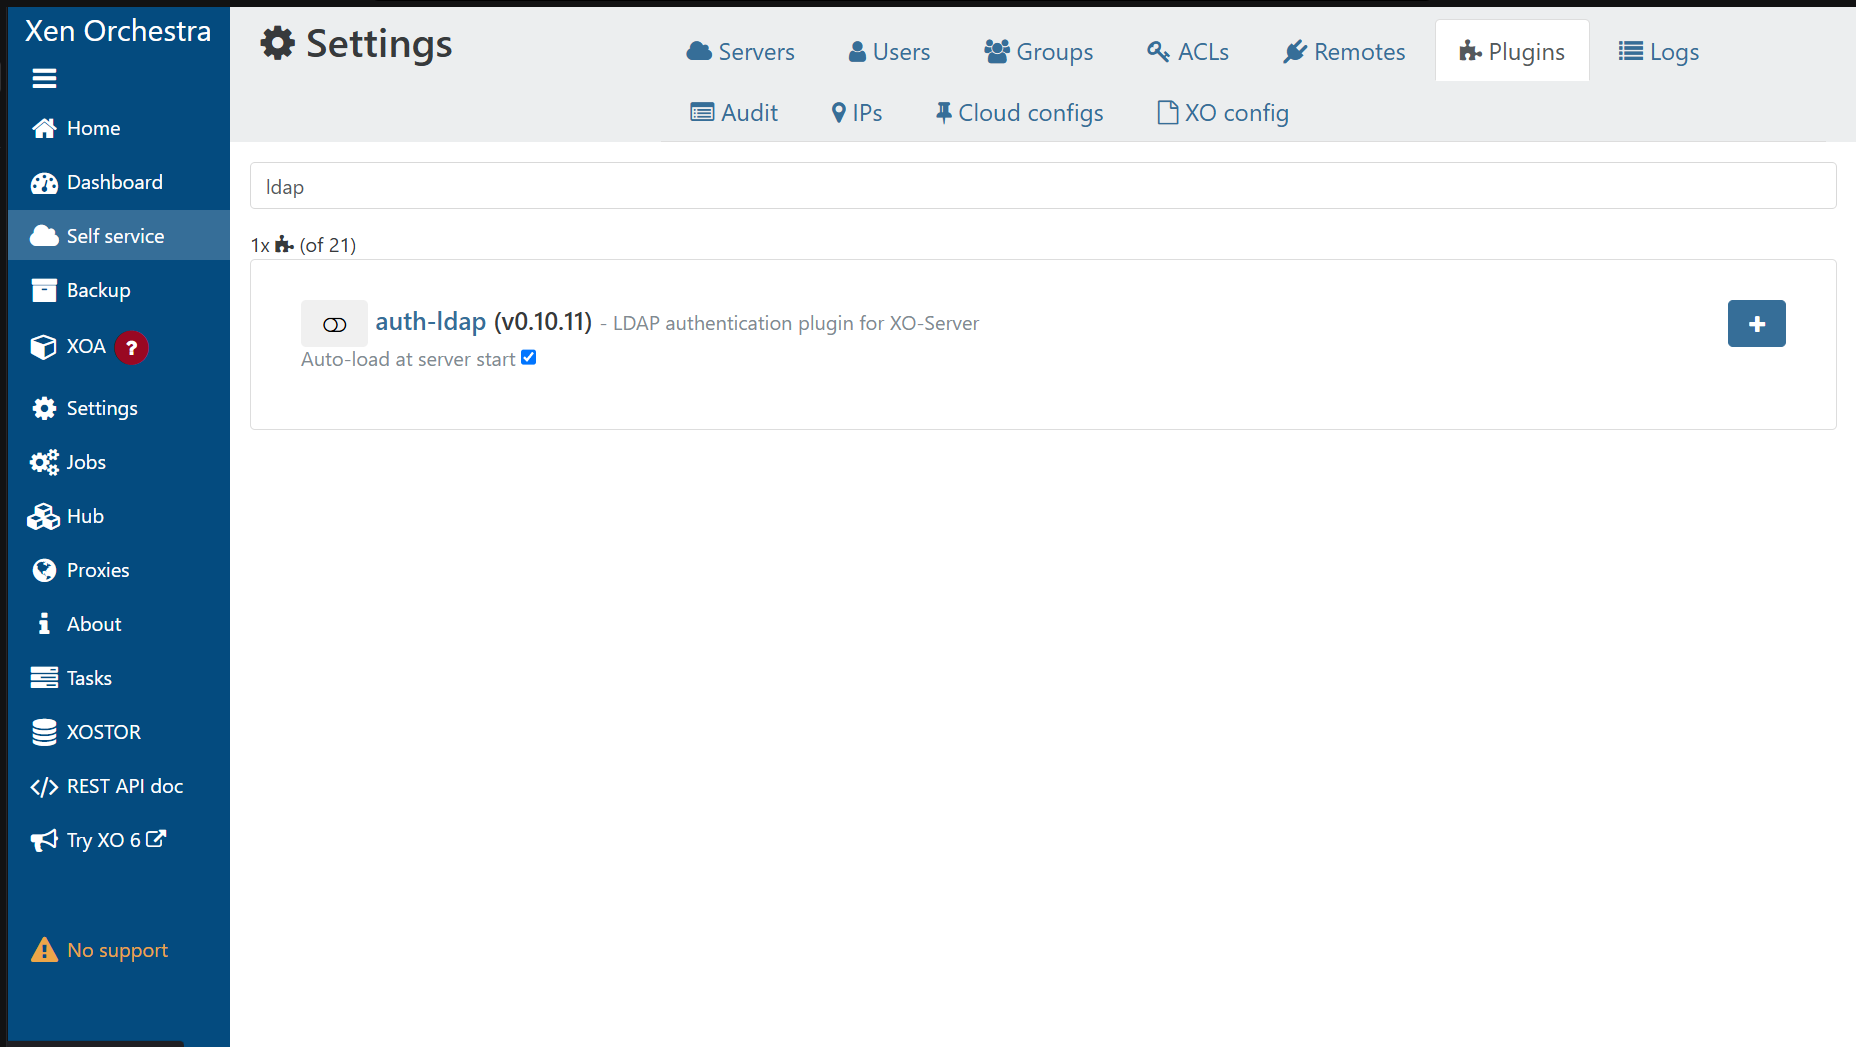
\includegraphics[width=0.8\textwidth]{mainmatter/II-desarrollo-metodologico/implementacion/imagenes/complemento-ldap-xen-orchestra.png}
	\caption{Complemento \acs{LDAP} disponible en Xen Orchestra}
	\label{fig:complemento-ldap-xen-orchestra}
\end{figure}

Para iniciar la configuración del complemento, el primer parámetro que se establece es la \ac{URI} del servidor \ac{LDAP}, la cual permite definir la dirección y el puerto mediante los que Xen Orchestra establece la comunicación con el servicio de directorio. En este caso, se utiliza la \ac{URI} \nolinkurl{ldap://ipa.grid.uniquindio.edu.co:389}, correspondiente al punto de acceso \ac{LDAP} definido para la infraestructura. Esta dirección permite que el complemento realice las consultas de autenticación contra el servicio de directorio a través de la identidad establecida para la infraestructura. La configuración de la \ac{URI} del servidor \ac{LDAP} en el complemento se muestra en la \autoref{fig:configuracion-uri-ldap-xen-orchestra}.

\begin{figure}[H]
	\centering
	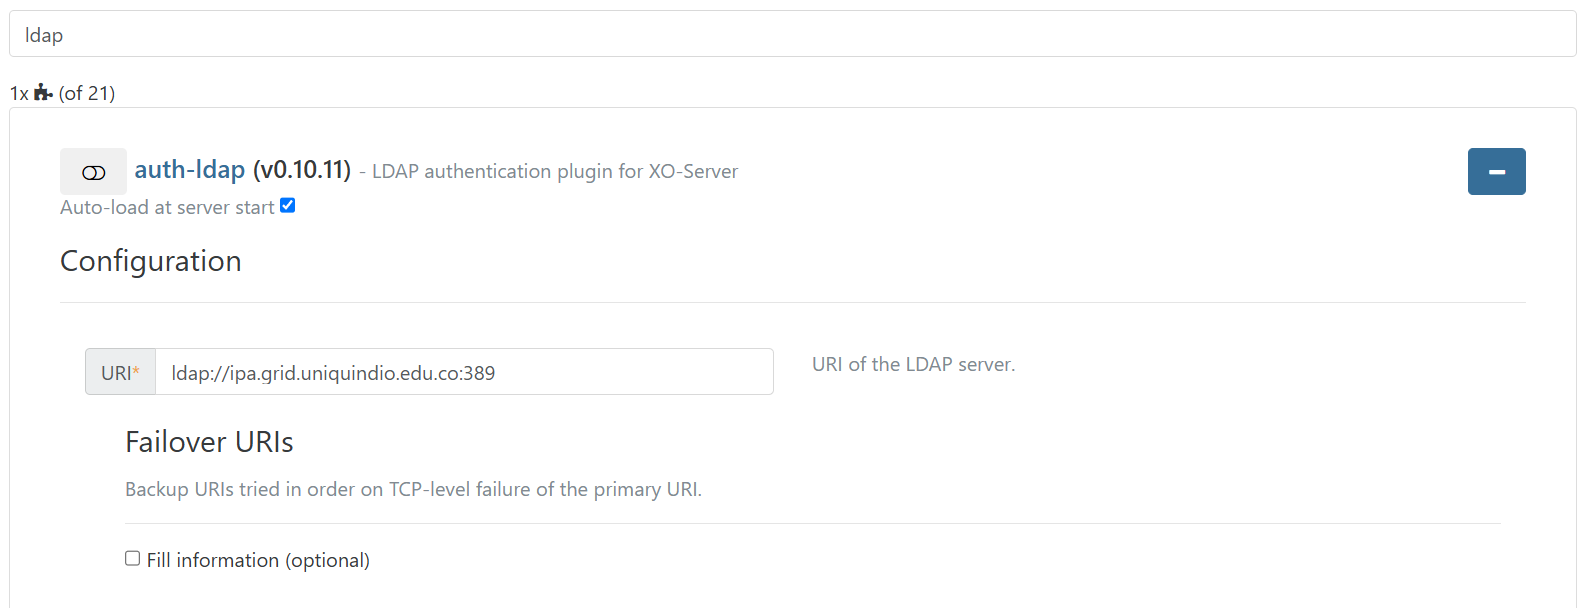
\includegraphics[width=0.8\textwidth]{mainmatter/II-desarrollo-metodologico/implementacion/imagenes/configuracion-uri-ldap-xen-orchestra.png}
	\caption{Configuración de la \acs{URI} del servidor \acs{LDAP} en el complemento de Xen Orchestra}
	\label{fig:configuracion-uri-ldap-xen-orchestra}
\end{figure}

Posteriormente, se configuraron los parámetros relacionados con la seguridad de la conexión y el ámbito de búsqueda dentro del directorio. En primer lugar, se estableció la ruta /home/node/ca.crt correspondiente al certificado de la autoridad certificadora de FreeIPA, el cual será utilizado para validar el certificado presentado por el servidor \ac{LDAP}. Para mantener la verificación de la identidad del servidor, se habilitó la opción Check certificate. Asimismo, se activó Use StartTLS, permitiendo que la conexión inicialmente establecida mediante \ac{LDAP} sea protegida mediante \ac{TLS}.

Finalmente, se definió como base del directorio el \ac{DN} \nolinkurl{dc=grid,dc=uniquindio,dc=edu,dc=co}. Este valor determina el punto de inicio dentro del árbol \ac{LDAP} a partir del cual el complemento realizará las búsquedas de usuarios y grupos. La combinación de estos parámetros permite establecer una conexión \ac{LDAP} cifrada y validar la identidad del servidor antes de realizar las consultas al directorio. La configuración del certificado, la seguridad \ac{TLS} y la base del directorio se observa en la \autoref{fig:configuracion-tls-base-xen-orchestra}.

\begin{figure}[H]
	\centering
	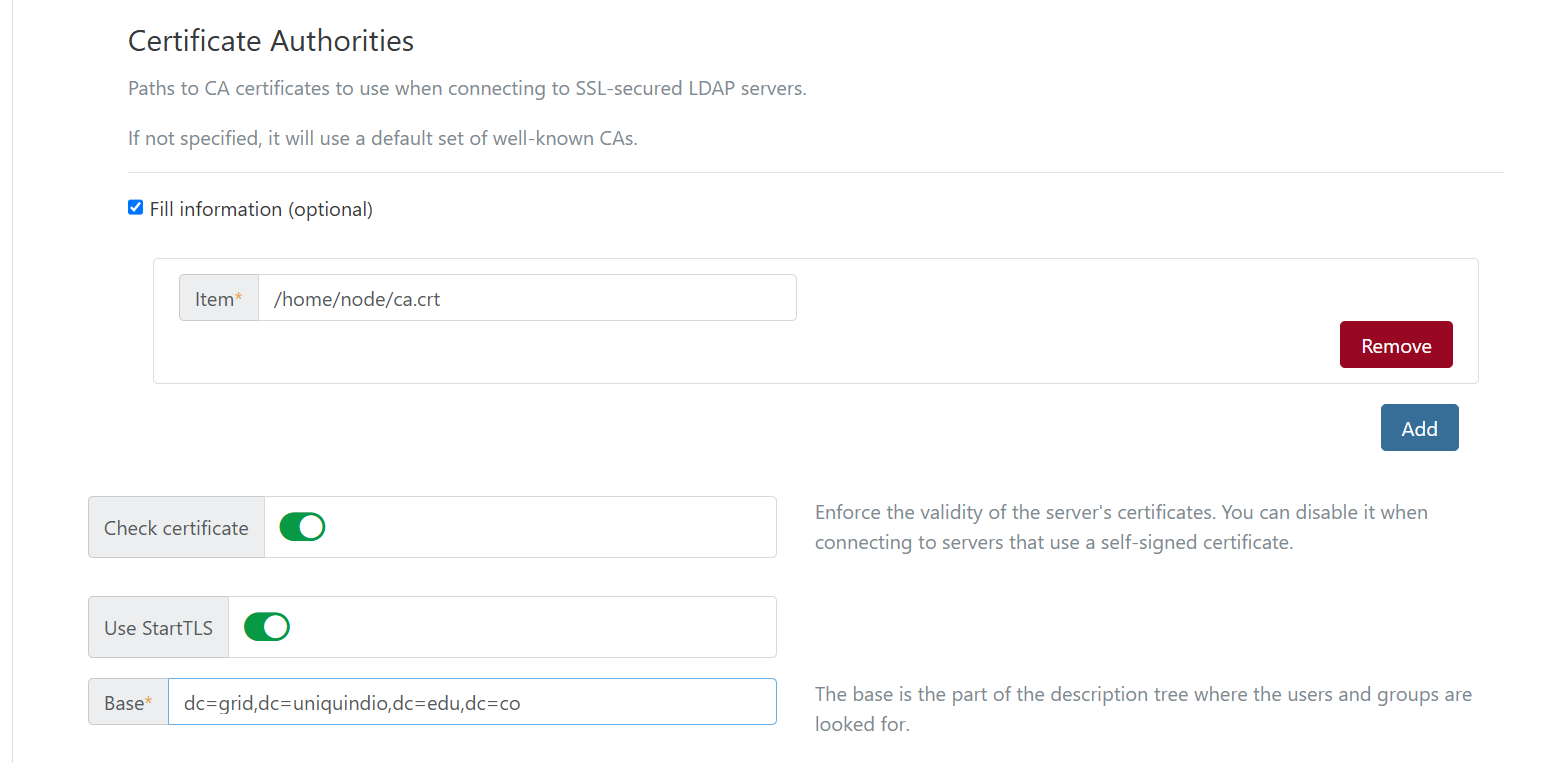
\includegraphics[width=0.8\textwidth]{mainmatter/II-desarrollo-metodologico/implementacion/imagenes/configuracion-tls-base-xen-orchestra.png}
	\caption{Configuración del certificado, seguridad \acs{TLS} y base del directorio \acs{LDAP} en Xen Orchestra}
	\label{fig:configuracion-tls-base-xen-orchestra}
\end{figure}

A continuación, se configuraron las credenciales que utilizará el complemento para realizar las consultas en el directorio \ac{LDAP} antes de localizar el registro correspondiente al usuario que intenta autenticarse. Para ello, se definió el \ac{DN} de la cuenta de servicio svc-xenorchestra, previamente creada para la integración con Xen Orchestra, junto con su respectiva contraseña. Esta cuenta permite realizar las búsquedas necesarias dentro del directorio sin utilizar las credenciales del usuario que posteriormente se autentica.

Adicionalmente, se configuró el filtro de usuario, mediante el cual se establece la condición que debe cumplir la cuenta para ser considerada durante el proceso de autenticación. En este caso, el filtro combina la identificación del usuario proporcionada por Xen Orchestra con su pertenencia al grupo xenorchestra, permitiendo que únicamente los usuarios autorizados para este servicio sean considerados por el complemento. La configuración de las credenciales y el filtro de búsqueda de usuarios se presenta en la \autoref{fig:configuracion-credenciales-filtro-xen-orchestra}.

\begin{figure}[H]
	\centering
	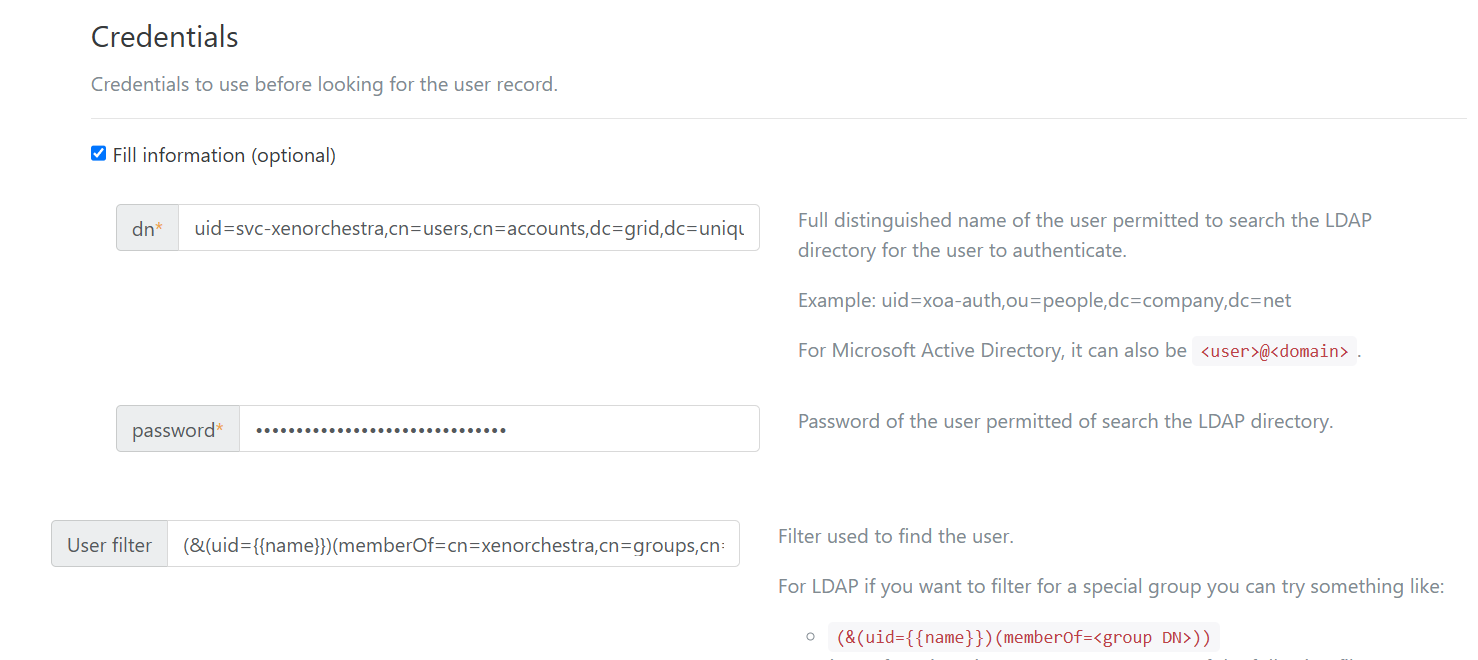
\includegraphics[width=0.8\textwidth]{mainmatter/II-desarrollo-metodologico/implementacion/imagenes/configuracion-credenciales-filtro-xen-orchestra.png}
	\caption{Configuración de las credenciales y filtro de búsqueda de usuarios \acs{LDAP} para Xen Orchestra}
	\label{fig:configuracion-credenciales-filtro-xen-orchestra}
\end{figure}

Finalmente, se configuró el atributo que permite identificar de forma única a los usuarios de \ac{LDAP} dentro de Xen Orchestra. Para este propósito, se estableció el atributo uid, utilizado para asociar cada cuenta del directorio con su correspondiente usuario en la plataforma. Asimismo, se mantuvieron sin configurar las opciones de sincronización de grupos y dominios adicionales, debido a que la integración implementada no requiere importar los grupos de FreeIPA directamente en Xen Orchestra ni utilizar dominios \ac{LDAP} adicionales.

Una vez definidos los parámetros necesarios, se procedió a guardar la configuración del complemento mediante la opción \textit{Save configuration}, dejando establecida la conexión entre Xen Orchestra y el servicio de directorio FreeIPA. Los parámetros finales de la configuración del complemento \ac{LDAP} y la opción para guardar la configuración se presentan en la \autoref{fig:configuracion-final-ldap-xen-orchestra}.

\begin{figure}[H]
	\centering
	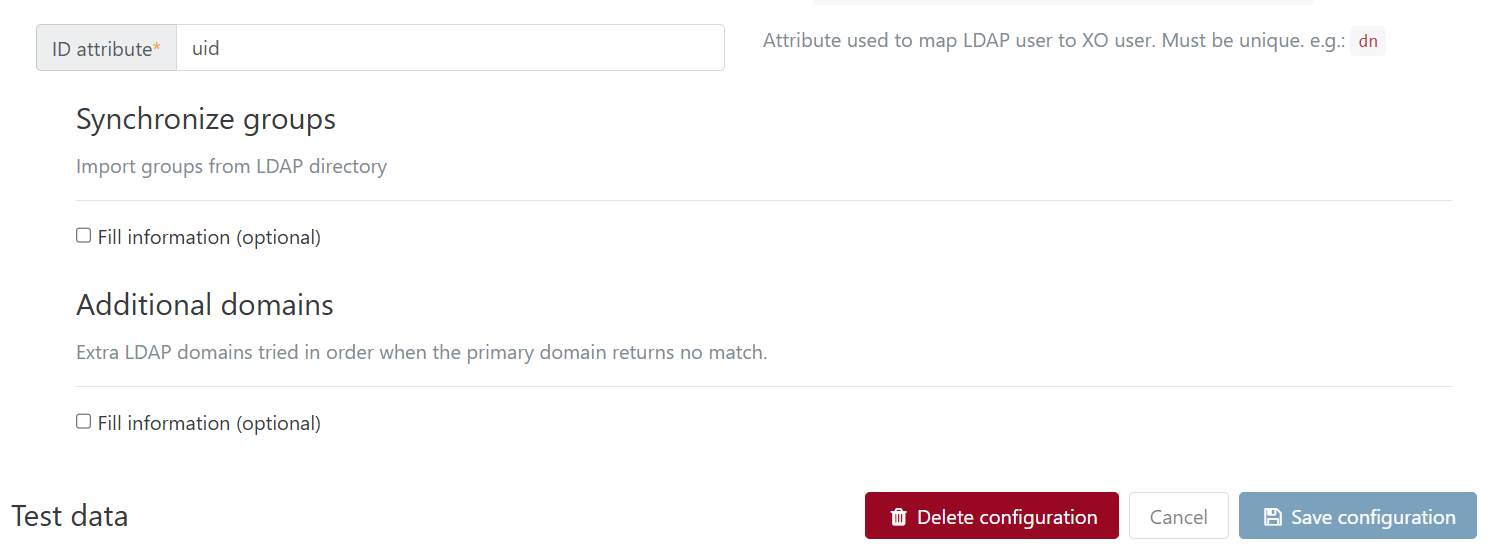
\includegraphics[width=0.8\textwidth]{mainmatter/II-desarrollo-metodologico/implementacion/imagenes/configuracion-final-ldap-xen-orchestra.png}
	\caption{Configuración final del complemento \acs{LDAP} en Xen Orchestra}
	\label{fig:configuracion-final-ldap-xen-orchestra}
\end{figure}

Finalmente, una vez completada la configuración del complemento, se procedió a activar el plugin \ac{LDAP} para poder realizar las pruebas de autenticación. Para ello, se utilizaron los datos de prueba disponibles en la sección \textit{Test data}, donde se ingresaron las credenciales de un usuario de FreeIPA y posteriormente se ejecutó la opción \textit{Test plugin}. Esta prueba permite comprobar el funcionamiento del complemento una vez habilitado y verificar que podía procesar correctamente las credenciales suministradas. Como resultado, Xen Orchestra mostró el mensaje \textit{“The test appears to be working”}, confirmando que la configuración realizada permitía establecer correctamente la comunicación y autenticación mediante \ac{LDAP}.

Los datos utilizados para la prueba se presentan en la \autoref{fig:datos-prueba-ldap-xen-orchestra}, mientras que el resultado satisfactorio obtenido se muestra en la \autoref{fig:resultado-prueba-ldap-xen-orchestra}.

\begin{figure}[H]
	\centering
	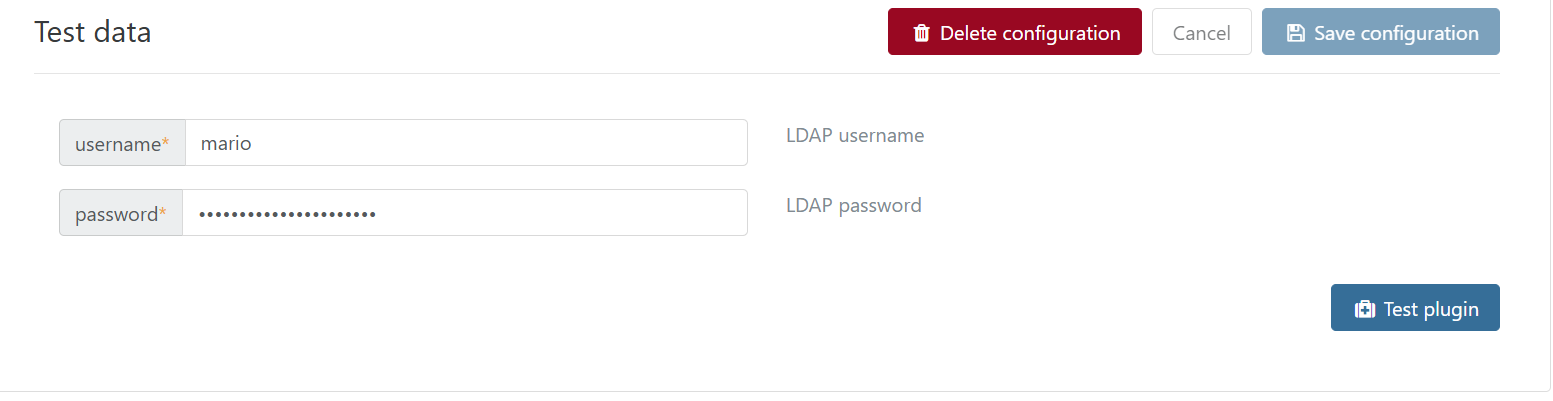
\includegraphics[width=0.8\textwidth]{mainmatter/II-desarrollo-metodologico/implementacion/imagenes/datos-prueba-ldap-xen-orchestra.png}
	\caption{Datos utilizados para la prueba del complemento \acs{LDAP} en Xen Orchestra}
	\label{fig:datos-prueba-ldap-xen-orchestra}
\end{figure}

\begin{figure}[H]
	\centering
	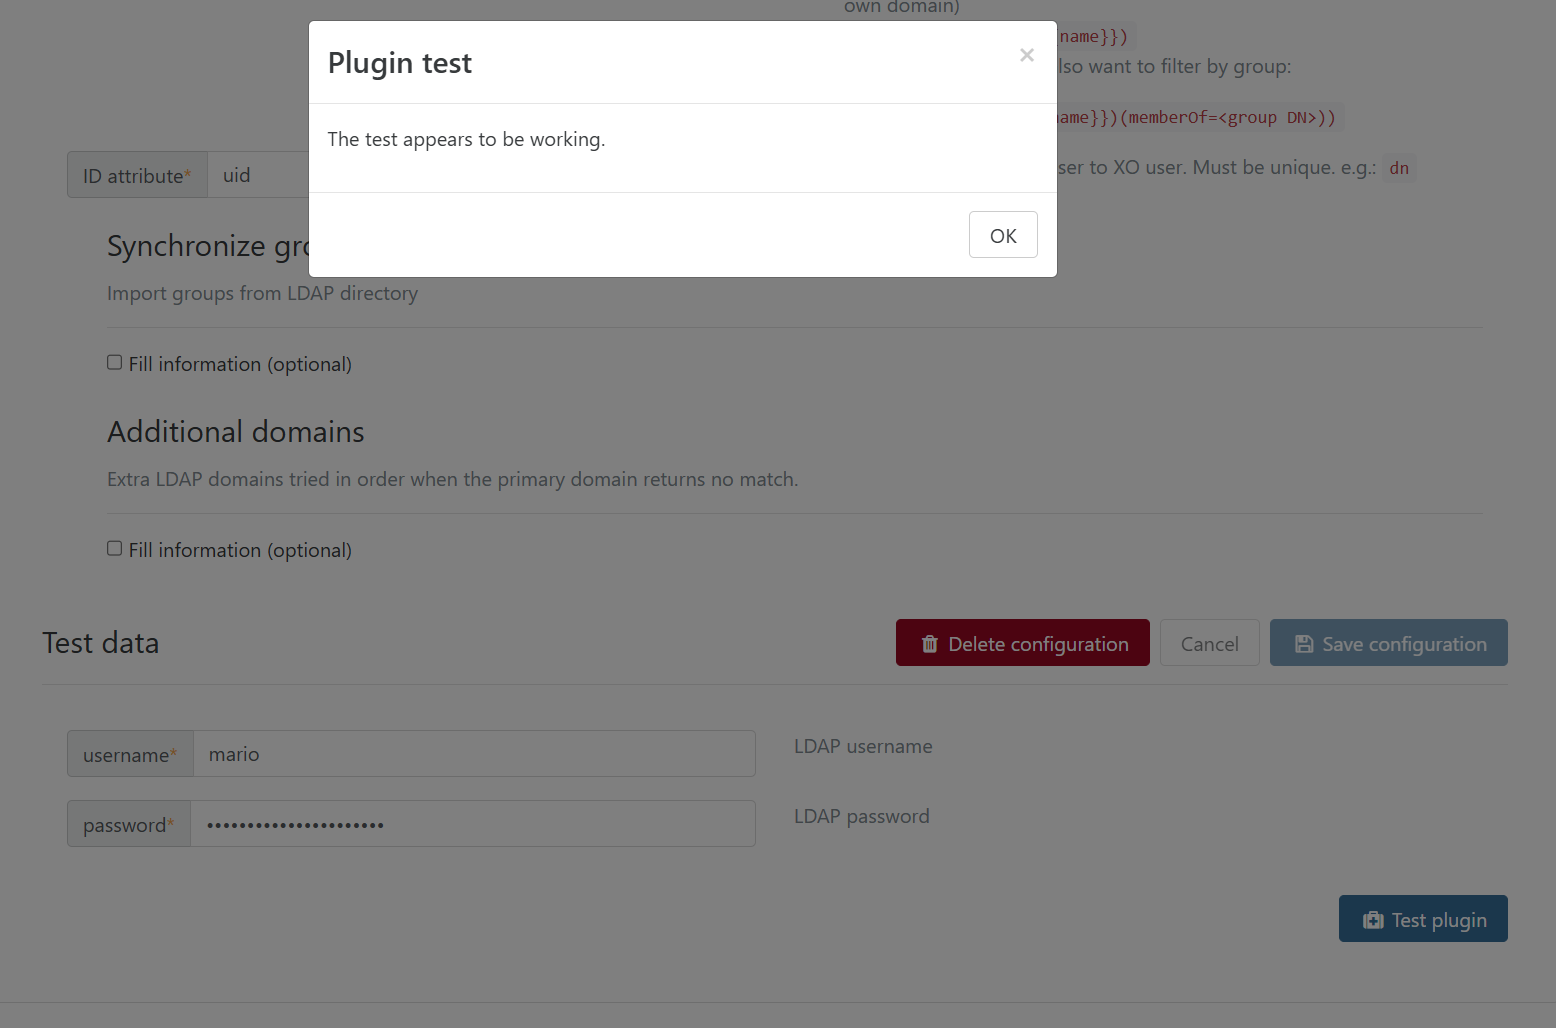
\includegraphics[width=0.8\textwidth]{mainmatter/II-desarrollo-metodologico/implementacion/imagenes/resultado-prueba-ldap-xen-orchestra.png}
	\caption{Resultado de la prueba de funcionamiento del complemento \acs{LDAP} en Xen Orchestra}
	\label{fig:resultado-prueba-ldap-xen-orchestra}
\end{figure}
